\documentclass[Space_Shuttle_Vessel_Manual.tex]{subfiles} 
\begin{document}

\section{SSV SYSTEMS}
\begin{multicols*}{2}
\renewcommand{\cfttoctitlefont}{\bf}
\localtableofcontents
\noindent
\\
This section discusses in greater detail some of the Space Shuttle systems that are currently simulated.\\
For better organization, the information about Payloads is provided in section \ref{sec:payloads}. In addition, information about the Upper Stages is located in section \ref{sec:upper-stages}.
\\
\\
These are not meant to provide all information about the real Space Shuttle systems, but instead to provide a working knowledge required to understand what is happening in the simulation.
\end{multicols*}


\subsection{Data Processing System (DPS)}
\begin{multicols*}{2}
\renewcommand{\cfttoctitlefont}{\bf}
\localtableofcontents
\noindent
\\
The DPS consists mainly of the General Purpose Computers (GPCs), the software that runs in them, and several Multiplexer/Demultiplexers (MDMs), along with a few other systems. The 11 MDUs (Multifunction Display Units) are also part of the DPS.
\subsubsection{GPCs}
The real Space Shuttle has 5 identical computers. Up to 4 of the 5 GPCs run the Primary Avionics Software System (PASS). The remaining computer runs the Backup Flight System (BFS). The PASS software is further divided into 3 Major Functions: \textit{GNC} (Guidance, Navigation \& Control), \textit{SM} (Systems Management) and \textit{PL} (Payload) software. The \textit{GNC} software is responsible for controlling the orbiter during flight. During critical phases of flight, such as launch and entry, multiple GPCs will run the PASS \textit{GNC} software simultaneously; this provides redundancy if one of the GPCs fails. The \textit{SM} software monitors various orbiter systems. The \textit{PL} software is not used during flight. The BFS was written separately from the PASS, and implements a subset of the PASS \textit{GNC} functions, along with SM functions during ascent and entry. The BFS is meant to be used in the event of a PASS failure.\\
\\
Each major function is divided into multiple OPS. Each \textit{GNC} OPS represents a different phase of flight. OPS 1 is used for launch, OPS 2 is used on-orbit, and OPS 3 is used for deorbit and entry. The GPC only has enough memory to store one OPS at a time, so the PASS software is divided into multiple memory configurations. Each memory configuration contains one OPS (except for MC 1, which is used during launch, and contains both OPS 1 (launch) and OPS 6 (RTLS)). To change from one OPS to another, the appropriate memory configuration has to be loaded onto the GPCs. Each OPS is further divided into Major Modes, which relate to specific phases of the mission. For example, OPS 2 (on-orbit) has 2 Major Modes: MM 201 (orbit coast) and MM 202 (Mnvr Exec). MM 202 is used for performing OMS burn, while MM 201 is used otherwise.\\
In \textit{SM} OPS 2, MM 201 is the main major mode for on-orbit SM operations, while MM 202 is used only to control PLBD opening and closing.\\
\\
At the moment, SSV simulates the PASS \textit{GNC} software in GPC-1 and PASS \textit{SM} software in GPC-2. Because GPC-2 is always running the SM software, it should be kept in OPS 0 for all phases of flight, except orbit. Loading different memory configurations into the GPCs is not simulated. SSV assumes only one GNC GPC is running, and does not simulate multiple GPCs performing the same operations as part of a redundant set, and does not simulate a common set. No major mode in GNC OPS 6 is currently supported. In the \textit{SM} GPC, only the "PL BAY DOORS" and "PL RETENTION" (DISP 97) displays are operational.\\
The "Maj Func" switches control which GPC (\textit{GNC} or \textit{SM}) is driving the associated MDU display, as well as the destination of the associated keyboard inputs.

\subsubsection{Multiplexer/Demultiplexer (MDMs)}
The GPCs get much of their data from Multiplexer/Demultiplexer (MDMs), which gather and digitize sensor readings and switch positions. Commands from the GPCs to several electrical motors, valves or lights are also routed thru the MDMs.\\
Several of the MDMs are implemented in SSV, with many signals flowing thru them.


\subsubsection{Multifunction Display Units (MDUs)}
The shuttle originally had 4 CRT displays, and multiple analog instruments.
The CRTs allowed the crew to interact with the shuttle computers, while the analog instruments displayed subsystem status and flight instruments.
Starting with STS-101, the analog instruments were replaced with the MDUs.
The shuttle has 11 MDUs: CDR 1 and 2 on panel F6; CRT 1, 2, and 3, and MFD 1 and 2 on panel F7; PLT 1 and 2 on panel F8; CRT 4 on panel R11; and AFD 1 in the aft station.
In real life, the MDUs display either DPS displays, flight instrument displays, or subsystem status displays.
The flight instruments and subsystem status displays replace the analog instruments, while the DPS displays are almost identical to the CRT displays.\\
\\
In SSV, each MDU is an Orbiter Simulator MFD. CRT MFD, which is part of SSV, simulates the DPS displays. Section \ref{sec:dps-displays} describes the DPS displays that have been implemented so far.
The 3 subsystem status displays (\textit{OMS/MPS}, \textit{APU/HYD} and \textit{SPI}) have been implemented in CRT MFD.
The flight instrument displays are only partially implemented. All displays in the Ascent/Entry Primary Flight Display are working except for full functionality of the ADI and HSI.
\end{multicols*}

\subsection{DPS Displays}
\begin{multicols*}{2}
%\renewcommand{\cfttoctitlefont}{\bf}
%\localtableofcontents
\label{sec:dps-displays}
\noindent
\\
The NASA DPS Dictionary describes each display in detail. This section lists the displays that have been implemented so far and describes the differences between the real shuttle and the SSV implementation.


\subsubsection{ASCENT TRAJ}
\begin{figure}[H]
  \includegraphics[scale=0.5]{ASCENTTRAJ2.png}
  \caption{ASCENT TRAJ display}
  \label{fig:ASCENT_TRAJ}
\end{figure}
This display is used in GNC MM 102 and MM 103 to monitor the vehicle's trajectory during ascent. The DROOP ALT digital output is not being driven. The ITEMs on this display are related to abort options and are not supported by SSV.

\subsubsection{UNIV PTG}
This display is used in GNC MM 201, and is used to control the attitude of the orbiter. Most of the functions in this display have been implemented. ITEM 8 (TGT ID) only supports an entry of 2 at the moment, and ITEMS 9-13 are not supported. ITEM 20 (TRK) is not supported. Finally, ITEMs 22-24 (which affect how the attitude error is displayed) are not implemented.

\subsubsection{OMS MNVR EXEC}
This display is used in GNC MM 104 (OMS 1 MNVR EXEC), MM 105 (OMS 2 MNVR EXEC), MM 106 (OMS 2 MNVR COAST), MM 202 (ORBIT MNVR EXEC), MM 301 (DEORB MNVR COAST), MM 302 (DEORB MNVR EXEC) and MM303 (DEORB MNVR COAST). It is used mainly to perform OMS engine burns to change the shuttle's orbit.\\
When entering MM 104 and MM 105, the PEG-4 parameters for the OMS-1 and OMS-2 burns, respectively, are already filled with values defined in the mission configuration (see \ref{sec:mission-configuration}). OMS-1 automatic maneuver load is currently not implemented.\\
ITEMs 35-40 (ABORT TGT, FWD RCS and SURF DRIVE) have not been implemented yet.

\subsubsection{OVERRIDE}
\begin{figure}[H]
  \includegraphics[width=0.99\hsize]{OVERRIDE.png}
  \caption{OVERRIDE display}
  \label{fig:OVERRIDE}
\end{figure}
The GNC display OVERRIDE currently only has implemented the 3 ITEM entries associated with the SSME maximum throttle, ITEM 42 to override the Entry Roll Mode switch and ITEM 45 to control the AerojetDAP Wraparound mode.

\subsubsection{DAP CONFIG}
This display is used in GNC MM 201 and MM 202, and control the Digital Autopilot (DAP) settings. In real life, there are 15 DAP A configurations and 15 DAP B configurations; at any time, 1 DAP A and 1 DAP B configuration is active, and the crew selects between DAP A and B using the PBIs on Panels C3 and A6. Currently in SSV there is only 1 DAP A configuration and 1 DAP B configuration. As a result, ITEMS 1 and 2 (which select the active DAP A \& B configuration) are not implemented. Also ITEMs 3 and 4 (which, in real life, select a DAP configuration and load it into the EDIT column) simply select between loading DAP A and DAP B into the EDIT column.\\
Currently, the default DAP configurations are for the typical ISS flight as follows: DAP A is DAP A1 for Nominal usage, and DAP B is DAP B10 for Docking operations.

\subsubsection{REL NAV}
The REL NAV display is available in GNC OPS 2 for rendezvous navigation. Currently only ITEM 1 is available, which enables and disables rendezvous navigation. Attempting to enable rendezvous navigation, without a target vessel specified in the scenario file, will result in an Illegal Entry fault message being generated. When rendezvous navigation is enabled, the computed range and rate, and planar offset and rate to the target will be displayed.

\subsubsection{ORBIT TGT}
This display is used in GNC MM 201 and MM 202 to compute rendezvous burns. In real life, the state vectors for the rendezvous target are uploaded from Mission Control. In SSV, the name of the target vessel is defined in the mission file (see \ref{sec:mission-configuration}). It is then kept in the scenario file, allowing the target to be (manually) changed if there is more than one rendezvous target.\\
With non-spherical gravity disabled, the predictor match will always be zero.

\subsubsection{ENTRY TRAJ 1-5}
\begin{figure}[H]
  \includegraphics[scale=0.5]{ENTRYTRAJ1.png}
  \caption{ENTRY TRAJ display}
  \label{fig:ENTRY_TRAJ}
\end{figure}
These displays are used during GNC MM 304 to monitor the vehicle's entry trajectory and AerojetDAP parameters. Currently only the phugoid scale and data is not driven and only ITEM 2 is supported.

\subsubsection{VERT SIT 1-2}
\begin{figure}[H]
  \includegraphics[scale=0.5]{VERTSIT1.png}
  \caption{VERT SIT display}
  \label{fig:VERT_SIT}
\end{figure}
These displays are used during GNC MM 305 to monitor the vehicle's TAEM trajectory and AerojetDAP parameters. Currently only the Theta scale is not driven.

\subsubsection{HORIZ SIT}
\begin{figure}[H]
  \includegraphics[scale=0.5]{HORIZSIT.png}
  \caption{HORIZ SIT display}
  \label{fig:HORIZ_SIT}
\end{figure}
This GNC display is used during deorbit and entry to specify the landing site and monitor the position of the shuttle relative to the HAC and the runway.
The HORIZ SIT display in SSV is simplified compared to the real life version.
Currently only ITEMs 3, 4, 6, 7, 8, 39 and 41 are supported.
ITEM 41 selects the landing site, ITEMs 3 and 4 select either the primary or secondary runway. ITEM 6 downmodes from an overhead approach to a straight-in approach, ITEM 7 toggles between the Nominal Entry Point (NEP) or the Minimum Entry Point (MEP), ITEM 8 switches the aim point between nominal and close, and ITEM 39 switches between nominal, short and ELS (Emergency Landing Site) speedbrake configurations for final approach.
These parameters all affect the entry autopilot, so they should be set before Entry Interface (EI).\\
The 45 landing sites for a mission are defined in the mission file (see \ref{sec:mission-configuration} and \ref{sec:landing-sites}).


\end{multicols*}

\subsection{MEDS Displays}
\begin{multicols*}{2}
%\renewcommand{\cfttoctitlefont}{\bf}
%\localtableofcontents
\label{sec:meds-displays}

\subsubsection{A/E PFD}
\begin{figure}[H]
  \includegraphics[width=0.99\hsize]{AEPFD.png}
  \caption{A/E PFD}
  \label{fig:AE_PFD}
\end{figure}
The Ascent/Entry Primary Flight Director display shows several parameters relevant to Ascent and Entry. Currently during launch and on-orbit, the attitude error needles are not properly driven, so they are not to be fully trusted (they are fully functional during entry). The ADI is operating in LVLH mode only (with yaw always zeroed when using Orbiter's original graphics engine), so the \textit{ADI ATT} switches have no effect. During launch the HSI is not referenced from the target plane and the X-Trk value is not being driven.

\subsubsection{ORBIT PFD}
\begin{figure}[H]
  \includegraphics[width=0.99\hsize]{ORBITPFD.png}
  \caption{Orbit PFD}
  \label{fig:Orbit_PFD}
\end{figure}
The Orbit Primary Flight Director is used for on-orbit display of vehicle attitude. Currently the attitude error needles currently are not being driven properly, so they are not to be fully trusted. The ADI currently operates only in the LVLH mode only (with yaw always zeroed when using Orbiter's original graphics engine), so the \textit{ADI ATT} switches have no effect. The Aft MDU is not driving the rates and error needles according to the "Sense" switch, thus data will show like in the forward MDUs.
\end{multicols*}
%currently better for spacing
\begin{multicols*}{2}
\subsubsection{OMS/MPS}
\begin{figure}[H]
  \includegraphics[width=0.99\hsize]{OMSMPS.png}
  \caption{OMS/MPS display}
  \label{fig:OMS_MPS_MEDS}
\end{figure}
The OMS/MPS display provides information about various pressures in the OMS and MPS systems. The OMS He TK P and N2 TK P meters are not driven.

\subsubsection{APU/HYD}
\begin{figure}[H]
  \includegraphics[width=0.99\hsize]{HYDAPU.png}
  \caption{APU/HYD display}
  \label{fig:APU_HYD_MEDS}
\end{figure}
The APU/HYD display shows pressures, quantities and temperatures related to the hydraulic system. The APU H2O QTY \%, OIL IN TEMP $^\circ$F and HYDRAULIC QTY \% meters are not driven.

\subsubsection{SPI}
\begin{figure}[H]
  \includegraphics[width=0.99\hsize]{SPI.png}
  \caption{SPI display}
  \label{fig:SPI_MEDS}
\end{figure}
The SPI display shows the position of the Orbiter Vehicle's aerosurfaces.

\subsubsection{Maintenance}
The MEDS maintenance displays are currently not being driven.
\end{multicols*}



\begin{multicols*}{2}
\subsection{Caution \& Warning (C\&W)}
To verify correct vehicle operation, several hundreds of parameters are monitored by the Caution \& Warning system (C\&W), and visual and aural alerts are given to the crew when something is wrong. The C\&W is composed of 2 parts: the Primary C\&W, which is a hardware system, and the software-based Backup C\&W.\\
The Primary C\&W system compares sensor voltages to pre-defined limits to verify subsystem temperatures, pressures and other parameters. The Backup C\&W also checks several subsystem parameters, in addition to alerting the crew when an off-nominal situation occurs (e.g., detection of a SSME failure).\\
The Primary C\&W system alerts the crew via the C\&W light matrix on Panel F7 and Master Alarm lights, and also the Master Alarm sound. The Backup C\&W system alerts the crew with fault messages in the CRT displays, and relies on the Primary C\&W illuminate lights on Panel F7 and to generate the Master Alarm sound and Systems Management tone. The parameters of the Primary C\&W system can have their limits changed or have their checks inhibited via controls on Panel R13U.\\
Currently the Primary C\&W system only verifies the MPS He and Manifold pressures and the Hydraulic system pressures, and only a few Backup C\&W alerts exist.
\end{multicols*}



\begin{multicols*}{2}
\subsection{Orbiter Boom Sensor System (OBSS)}
After the Columbia accident, the Space Shuttle introduced the Orbiter Boom Sensor System (OBSS), to effectively extend the reach of the RMS, thus allowing the inspection of the TPS in areas that could not be checked with the RMS alone.
The OBSS has a sensor package on the tip to record TPS condition and 2 Grapple Fixtures (GF) for the RMS to maneuver it.\\
In the current implementation, the OBSS is completely passive.
%mention PWP attachment
\begin{figure}[H]
  \includegraphics[width=0.99\hsize]{OBSS.png}
  \caption{Orbiter Boom Sensor System}
  \label{fig:OBSS}
\end{figure}
\end{multicols*}



\begin{multicols*}{2}
\subsection{Launch Pads}
SSV can be launched from 2 launch sites: the 2 pads at Launch Complex 39 (LC39) at the Kennedy Space Center in Florida, from where all Space Shuttle missions were launched, and from Space Launch Complex 6 (SLC-6) at the Vandenberg Air Force Base in California, where polar-orbit missions were planned to be launched starting in 1986.
\begin{figure}[H]
  \includegraphics[width=0.99\hsize]{LC39.png}
  \caption{Launch Complex 39}
  \label{fig:LC39}
\end{figure}
\begin{figure}[H]
  \includegraphics[width=0.99\hsize]{SLC6.png}
  \caption{Space Launch Complex 6}
  \label{fig:SLC6}
\end{figure}
\noindent
Most pad structures are controlled automatically during the countdown, but manual control is available for all of them via a dialog window which is opened by the keys Ctrl+Space. Manual commands might be blocked to avoid structural interference, e.g., the GVA can only be moved if the GOX Vent Hood is raised.\\
\noindent
To accommodate the changes throughout the years, LC39 is available in 8 types$\colon$\\
$\Rightarrow$ 1981, the original STS-1 pad (not implemented yet, currently similar to the 1982 version);\\
$\Rightarrow$ 1982, new GVA GOX vent pipes;\\
$\Rightarrow$ 1983, RBUS (Rolling Beam Umbilical System) porch added;\\
$\Rightarrow$ 1985, RBUS added;\\
$\Rightarrow$ 1986, 'hypothetical' pad version with RBUS and OWP (Orbiter Weather Protection);\\
$\Rightarrow$ 1988, OWP added and RBUS removed;\\
$\Rightarrow$ 1995, hammerhead crane truss removed;\\
$\Rightarrow$ 2007, last pad iteration without the hammerhead crane and with a new lightning mast.\\
\end{multicols*}

\begin{multicols*}{2}
\subsection{Launch Control Center}
\noindent
The Launch Control Center (LCC) vessel controls the countdown clock, issues commands to the launch pad and Space Shuttle vehicle and monitors their status during the countdown. User interaction with the LCC vessel is done via the LCCMFD.
\\
The LCCMFD (Ctrl+T) allows the user to control the final 9 minutes of the countdown. Using the MFD buttons, the user can resume the countdown clock after a hold is called automatically due to violation of a Launch Commit Criteria parameter, and can also insert holds manually. In addition to the status of the final 5 hold points, the T0 time and countdown clock are also displayed. The countdown clock is also shown in the debug line (lower left corner of the window).
\\
The launch pad Firex systems are also controlled from the LCCMFD. Using the (Left/Right)Shift+1 keyboard keys, operation of the Orbiter SSME Water Deluge System (SSME Heatshield) is controlled. This system is activated automatically after a pad abort, and is manually shutdown. (Left/Right)Shift+2 and (Left/Right)Shift+3 control the operation of the LH2/LO2 T-0 Water Deluge System (T0 Umbilicals) and the Orbiter Skin Spray System (Orbiter Skin), respectively. The current status of the 3 systems is displayed in the LCCMFD.
\end{multicols*}


\begin{multicols*}{2}
\subsection{Crawler Transporter}
\noindent
The Crawler Transporter vessel allows the transfer of the MLP (with or without the Space Shuttle launch vehicle) from the VAB to the Launch Pad, and back. Currently all major functionalities of the Crawler are supported.
\begin{figure}[H]
  \includegraphics[width=0.99\hsize]{CT.png}
  \caption{Crawler Transporter}
  \label{fig:CT}
\end{figure}
\noindent
The Crawler Transporter is available in 2 versions$\colon$\\
$\Rightarrow$ a 1980 version, used for most of the Space Shuttle Program;\\
$\Rightarrow$ the later version, with modifications related to sound attenuation, among others.\\
\\

\subsubsection{Cabin selection}
The Crawler Transporter has 2 cabins from which it can be controlled$\colon$ Cabin-3 at the front, and Cabin-1 at the rear. The selection, or deselection, of a cabin for control is made by depressing the "CAB ACK" PBI on the right panel, and the selection state is indicated by the "Cab Selected" light. When only one cabin is selected, it will be in control and the "Cab In Control" light will be illuminated in the cabin in control.
\\

\subsubsection{Motion}
The Crawler Transporter motion is controlled by 3 mode PBIs and a speed control knob.\\
Forward motion is commanded by the FWD PBI, and aft motion is commanded by the REV PBI. The direction always referenced on the cabin in control. The NEUT PBI disengages the engine from the tracks.\\
The speed knob is controlled by the + and - NumPad keys, which will respectively increase and decrease the commanded speed. The actual Crawler speed is indicated in the top of the center panel.\\
The Crawler has a service brake, which is actuated by pressing the B key, and a parking brake controlled by the BRAKE PBI on the center panel.
\\

\subsubsection{Steering}
The Crawler Transporter steering is controlled with a steering wheel, located in the center console. The steering wheel is controlled by the 1 and 3 NumPad keys, for left and right turns respectively. Additionally, the 5 NumPad key can be used for immediate steering wheel centering.\\
The Steer Mode PBI, on the right console, controls the steering wheel scale$\colon$ the normal +/-6$^\circ$ setting provides the most direct control of the steering by allowing 6 degrees to be commanded, as labeled in the steering wheel; while the +/-2$^\circ$ option only allows a maximum of 2 degrees of steering to be commanded at full steering wheel deflection, thus allowing for more sensitive directional control.\\
The Crawler has different 3 modes of steering, selected by PBIs on the right console: Great Circle (G CIRC) mode allows the Crawler to go around corners by turning the forward drive trucks in the opposite direction to the aft drive trucks; Independent (INDEP) mode, allows independent control of each end of the Crawler by having each cabin controlling only the drive trucks on its end; Crab (CRAB) mode allows the Crawler to move diagonally, without changing the heading, to sort out any lateral misalignments with a target, by commanding all drive trucks in the same direction.\\
The desired steering angles of the drive trucks on each end of the Crawler are displayed on the right console, as is the actual steering input.
\\

\subsubsection{Jacking, Equalization and Leveling system}
The Jacking, Equalization and Leveling system (JEL) is comprised of 16 hydraulic cylinders, 4 in each corner of the Crawler, that are responsible for maintaining the Crawler Transporter leveled, and also allowing it to lift the MLP off its stands. Each hydraulic cylinder can be extended a maximum of 6 feet.\\
The AVERAGE HEIGHT gauge on the right console is showing the averaged height between all four corners. When the Crawler is exactly level (not ascending or descending the pad ramp) the gauge shows the extension all JEL cylinders.\\
Crawler jack-up is commanded by the Ctrl+K keys, and jack-down by the Ctrl+J keys. The Crawler can be commanded to 3 height levels, in order of increasing height$\colon$ (1) travel height, the normal height for Crawler travel; (2) docking height, the height to pickup and harddown the MLP; (3) clearance height, the maximum height to raise the MLP above the mounts.
\\

\subsubsection{Laser Docking System}
The Laser Docking System allows the driver to visualize the lateral alignment between the Crawler and its target (either the MLP or the mounts if the MLP is attached). It is the yellow rectangular box on top of the right console. None of the switches except for the CAB 1/3 switch, which allows the LDS display to switch between the receivers mounted on each end, so that the driver can correct any rotational misalignments without communicating with the driver in the opposing cab. It's a steer-to alignment system, so if the black alignment bar is on the right you need to steer to the right, and if it is on the left you need to steer to the left. The goal is to get the alignment bar in the very center of the display, for both Crawler ends.
\\

\subsubsection{Procedures and general notes}
Do note that the Crawler accelerates very much like a train so don't expect on the dime stop, always plan your speeds ahead especially when you are approaching your target (your speed should then be below 0.1 MPH).\\
Make sure you always plan your trajectory, as the Crawler has a slow response to steering inputs.\\
Attaching/detaching the MLP to the Crawler can only be done in the docking height. The proper procedure is to fully jack down the Crawler once the MLP has fully cleared the mounts either in the VAB or at the pad.
\\

\subsubsection{Compatibility}
The SSV Crawler is compatible with any launcher platform as long as the attachment point has the ID of XMLP. The attachment point on the launcher platform should be on the very bottom of the platform.
\\

\end{multicols*}

\begin{multicols*}{2}
\subsection{Landing Sites}
\label{sec:landing-sites}
\noindent

The landing sites for Space Shuttle end-of-mission landings were the Shuttle Landing Facility (SLF), Edwards Air Force Base (EAFB) and White Sands Space Harbor (WSSH). In addition, many runways in civilian airports and military air bases around the world were selected as Space Shuttle landing sites for abort or emergency landings.
\\
Several of these landing sites have been implemented in SSV, as Orbiter Simulator surface bases, and are available for use.
\\
The full list of landing sites are listed in "<Orbiter installation>\textbackslash Config\textbackslash SSV\_RunwayDB.csv", and also in the Landing tab of Mission Editor.
Table \ref{tab:LandingSites} shows the currently implemented landing sites that are part of the default landing site list.

\begin{table}[H]
  \centering
  \begin{tabularx}{225pt}{c | >{\centering\arraybackslash}p{70pt} | >{\centering\arraybackslash}p{45pt} | >{\centering\arraybackslash}p{45pt}}
    \textbf{SITE} & \textbf{Location} & \textbf{PRI RWY} & \textbf{SEC RWY} \\
    \hline
    1 & KSC & KSC 15 & KSC 33 \\
    2 & Ben Gerir & BEN 36 & BEN 18 \\
    3 & Moron & MRN 20 & MRN 02 \\
    4 & Zaragoza & ZZA 30L & ZZA 12R \\
    5 & Myrtle Beach & MYR 36 & MYR 18 \\
    12 & Ben Gerir & BEN 36 & BEN 18 \\
    13 & Moron & MRN 20 & MRN 02 \\
    14 & Zaragoza & ZZA 30L & ZZA 12R \\
    16 & Otis & FMH 32 & FMH 23 \\
    20 & St Johns & YYT 29 & YYT 11 \\
    21 & Gander & YQX 21 & YQX 31 \\
    22 & Banjul & BYD 32 & BYD 14 \\
    23 & Lajes & LAJ 15 & LAJ 33 \\
    24 & Vandenberg & VBG 30 & VBG 12 \\
    26 & Shannon & INN 06 & INN 24 \\
    28 & Koln/Bonn & KBO 14L & KBO 32R \\
    29 & Istres & FMI 33 & FMI 15 \\
    32 & Diego Garcia & JDG 31 & JDG 13 \\
    33 & Amberley/Tindall & AMB 15 & PTN 14 \\
    34 & Yokota & JTY 36 & JTY 18 \\
    36 & Bermuda & BDA 30 & BDA 12 \\
    38 & Mataveri & EIP 28 & EIP 10 \\
    39 & Hao & HAO 12 & HAO 30 \\
    42 & White Sands & NOR 17 & NOR 23 \\
    43 & White Sands & NOR 05 & NOR 35 \\
    44 & Edwards & EDW 15 & EDW 18L \\
    45 & Edwards & EDW 22 & EDW 04
  \end{tabularx}
  \caption{Default Landing Site Table}
  \label{tab:LandingSites}
\end{table}


\noindent
\begin{figure}[H]
  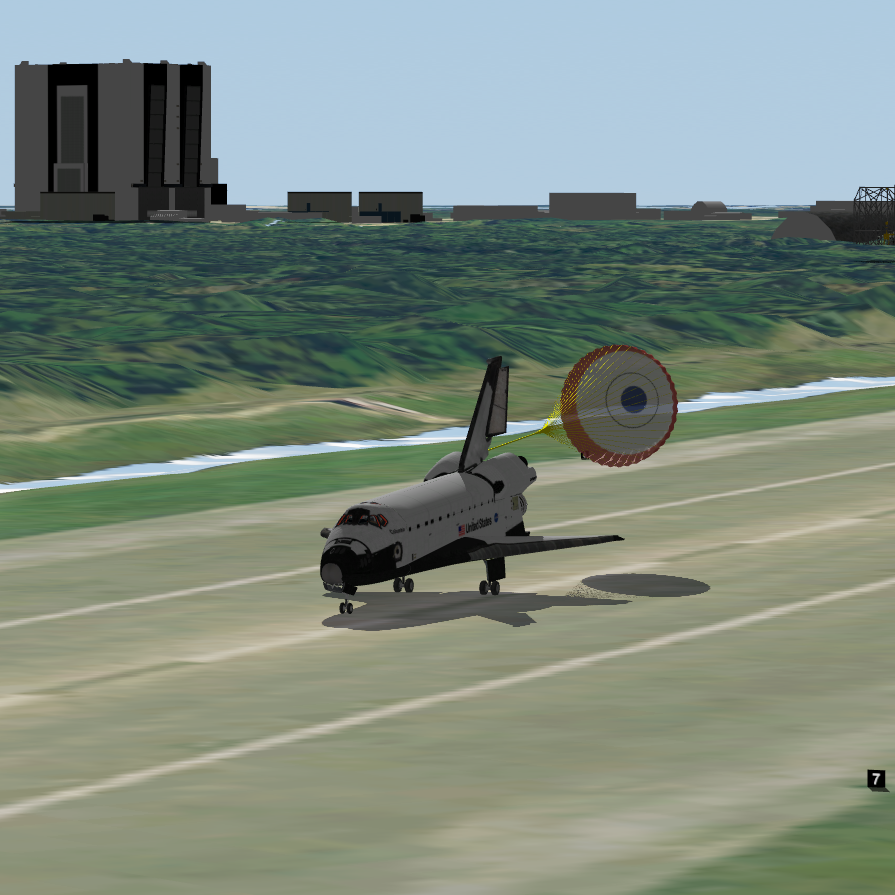
\includegraphics[width=0.99\hsize]{ksclanding.png}
  \caption{Shuttle Landing Facility (SLF)}
  \label{fig:SLF}
\end{figure}


\noindent
\begin{figure}[H]
  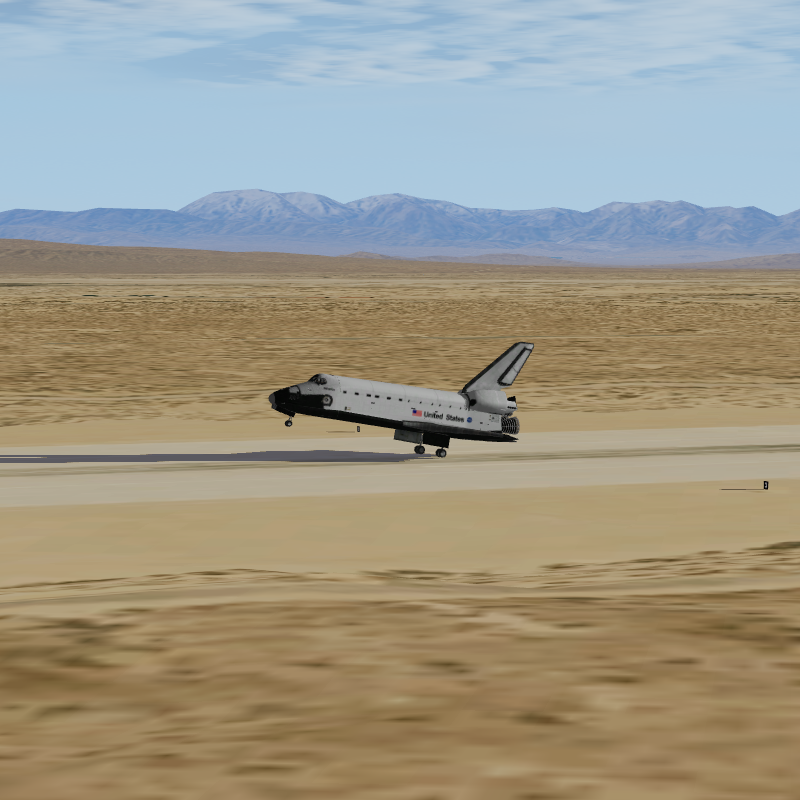
\includegraphics[width=0.99\hsize]{edwlanding.png}
  \caption{Edwards Air Force Base (EDW)}
  \label{fig:EDW}
\end{figure}

\end{multicols*}
\end{document}
